\documentclass[11pt]{article}

\title{\textit{morderstats.py} Documentation}
\date{\today}

\usepackage{framed}
\usepackage{listings}
\usepackage{graphicx}
\usepackage{hyperref}

\lstset{
	language=bash,
	breaklines=true	
}

\begin{document}
\maketitle

This document describes how to use the program \textit{morderstats.py} to generate multivariate prediction regions from forecast data. The name \textit{morderstats} is short for \textit{multivariate order statistics} and indicates the capability of this program to produce multivariate information using different methods and then order them based on certain metrics. Currently the only methods of producing prediction regions are by using the Mahalanobis distance, Direct Convex Hull Peeling, and Halfspace Convex Hull Peeling.

\section{Required Modules}

\textit{morderstats.py} is dependent on the entire scipy stack. This is most easily obtainable by downloading and installing the most recent Anaconda distribution and can be found at  \url{https://www.continuum.io/downloads}. Alternatively, one can install the modules \textit{numpy}, \textit{scipy}, \textit{matplotlib}, and \textit{pandas} by using the command \texttt{pip install <module>} and replacing \texttt{<module>} with the appropriate module name. To achieve complete functionality of the program, you will need to have installed \textit{scipy} 0.19 or later.

There is an alternate implementation of the program which is dependent on the module \textit{pyhull}. This can be installed using the command \texttt{pip install pyhull}.

\section{Formatting the Input Data}

To properly use this program, the input file should simply contain the raw data. Each row should represent an individual point in multiple dimensions, and each column should represent a dimension. The following text demonstrates how to properly format the file:

\begin{framed}
	\noindent
\\
101,101\\
102,103\\
102,107\\
107,110\\
\end{framed}

\section{Configuring Options}

To actually execute the program, the user must create an options file which specifies the various options required for running the program. For clarity purposes, we will refer to this file as \texttt{morderstats\_exec.txt} but note that this file can be given any name.

This file must start with the following line verbatim:
\begin{center}
	\texttt{command/exec morderstats.py}
\end{center}
This specifies that the options file is for executing \textit{morderstats.py}

There are four options that are mandatory and one option that is optional.
The first option that must be set is \texttt{--sources-file} which specifies the data file with which you wish to compute multivariate order statistics.
The second option that must be set is \texttt{--method} which designates which method you wish to use for producing the prediction regions.
If set to \textit{mahal}, then regions will be computed using the mahalanobis distance.
If set to \textit{halfspace}, then regions will be computed using the halfspace peeling algorithm.
If it is set to \textit{direct}, then regions will be computed using the direct convex hull peeling algorithm.

The option \texttt{--write-file} must be set and designates the name of the text file which will contain information about the prediction regions computed.
The option \texttt{--write-directory} must also be set and designates the name of the directory to contain all files produced by \textit{morderstats}.

The option \texttt{--alpha} is optional and designates the desired proportion of points to be outside the prediction region. If unspecified and \texttt{--method} is set to \textit{mahal}, then regions will be computed for $\alpha = 0.01,0.02,\ldots,0.99$. If it is unspecified and the \texttt{--method} is set to either \textit{halfspace} or \textit{direct}, then the entire sequence of convex hulls will be computed by the respective method.

The following figure demonstrates an example for how the options file could be written:

\begin{framed}
	\lstinputlisting{morderstats_exec.txt}
\end{framed}

Once the options file is written, \textit{morderstats.py} can be executed with the following command:
\begin{center}
	\texttt{python runner.py morderstats\_exec.txt}
\end{center}

If you gave your options file a different name than \textit{morderstats\_exec.txt}, then you can change the command to use the appropriate name.

\section{Output Files}
After running, the program will output data files and plots in the directory specified in the options file. The first will be a text file named \texttt{regions.csv} which contains the points for the defining polygon of the convex hull for the specified alpha level and method of producing the prediction region. It will also contain the proportion of points outside the region as well as the volume of the region. Here is an example of what this file may look like:

\begin{framed}
	\lstinputlisting{example_write_file.csv}
\end{framed}

The second file produced will be a plot of the region or regions.
The following figure is an example plot that was produced by \textit{morderstats}

\begin{center}
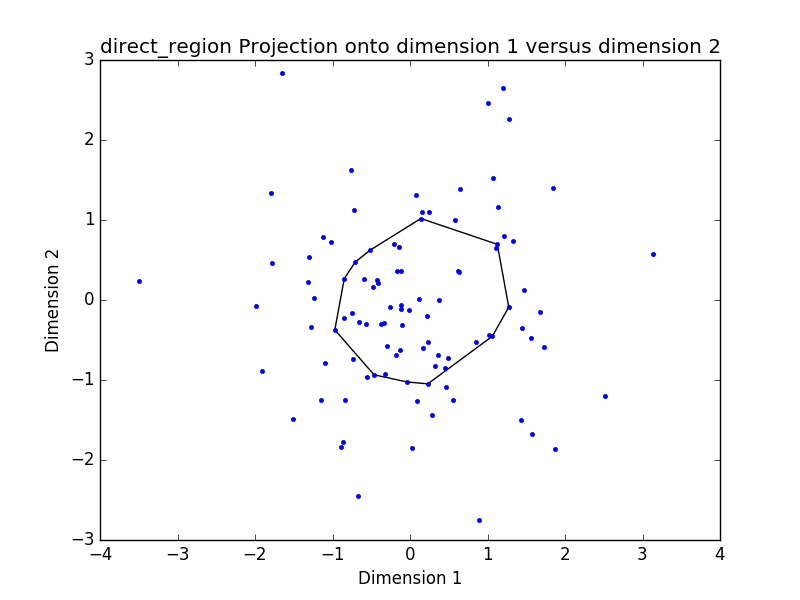
\includegraphics[height=200pt]{direct_region1vs2.png}
\end{center}

\section{Testing}
This program comes with an associated test suite for testing if \textit{morderstats} or the associated modules in \textit{pint} function properly.
To run this tester, simply execute the following command in the terminal in the \textit{pint} directory:
\begin{center}
	\texttt{python tester.py}
\end{center}

\end{document}